\section{Задание 1}

Ликвидируйте перегрузку ресурсов в проекте.

В данный момент в проекте наблядается перегрузка 3 ресурсов:
\begin{enumerate}
	\item Системный аналитик;
	\item Художник;
	\item Технический писатель;
\end{enumerate}

Перегрузка произошла из за одновременного выполняния задач.

Для устранения перегрузки можно использовать:
\begin{enumerate}
	\item изменить календарь работы ресурса;
	\item назначить ресурс на неполный рабочий день;
	\item изменить профиль назначения ресурса;
	\item применить выравнивание;
	\item разбить задачу на подзачи и перекрыть по времени выполнения;
\end{enumerate}

Выполним автовыравнивание \ref{fig:lab311}.
\begin{figure}[H]
	\centering
	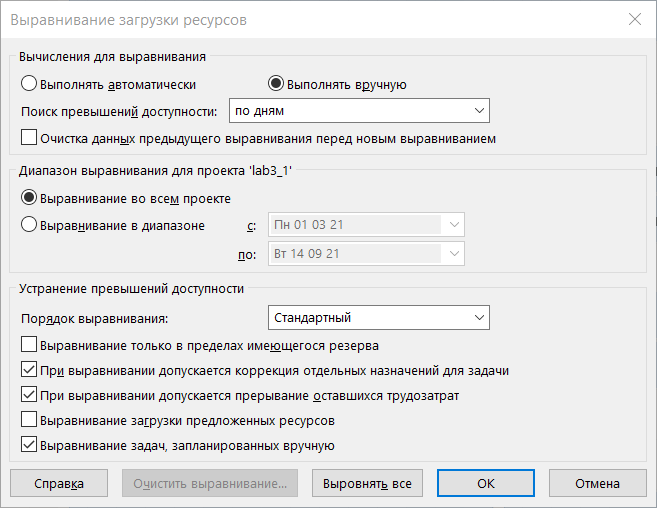
\includegraphics[width=0.7\linewidth]{src/lab3_1_1}
	\caption{Выравнивание}
	\label{fig:lab311}
\end{figure}

В результате выравнивания перегрузка ресурсов была устранена.

\section{Задание 2}
Подзадачи:
\begin{enumerate}
	\item отразите в плане проекта проведение еженедельного совещания по
	средам с 10 до 11 утра \ref{fig:lab321}
	\item привлеките к участию в совещании всех специалистов, кроме
	наборщиков данных и программистов №1 - 4 (их интересы на совещании
	представляет ведущий программист);
	\item устраните перегрузку ресурсов;
	\item в случае превышения бюджета и сроков реализации проекта проведите
	оптимизацию временных и финансовых параметров проекта.
\end{enumerate}

\begin{figure}[h]
	\centering
	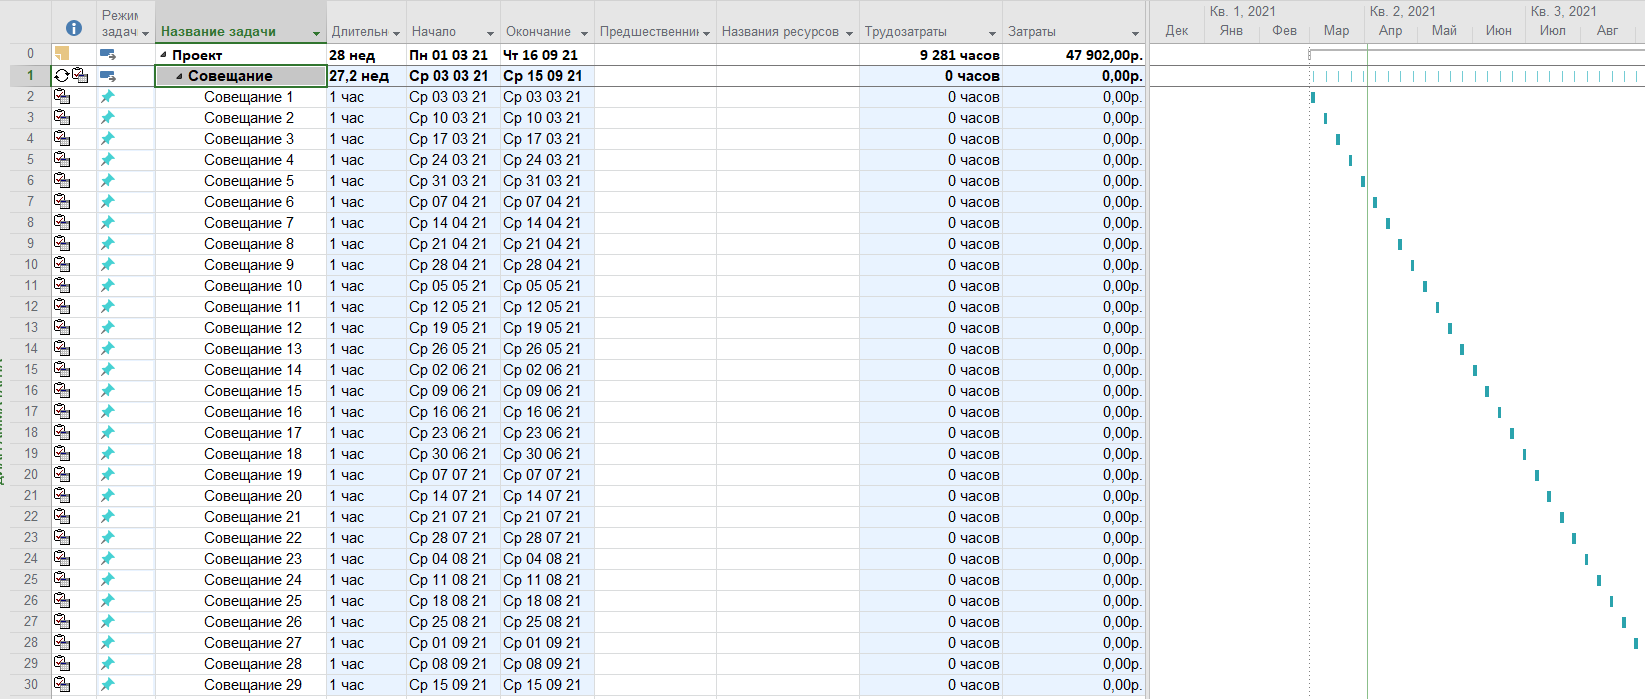
\includegraphics[width=0.7\linewidth]{src/lab3_2_1}
	\caption{Совещание}
	\label{fig:lab321}
\end{figure}

После добавленя совещания, появилась перегрузка ресурсов и увеличение стоимости проекта с 47938р до 67997р.
Проведем повторное выравние ресурсов.
После проведения выравнивания ресурсов, мы можем видеть что задачи разбились на интервалы, между которыми встали совещания.
Данное действие привело к увеличению продолжительности до 28.68 недель.

Для того что бы снизить траты введем новую ставку на время совещания.
После введния норм затрат на совещание. Стоимость проекта уменьшилась до 48344р.
Теперь вернем проект в рамки установленных сроков.
Для этого на разработку модели ядра добавим программиста 2. Длительность проекта уже уменьшилась до 14.09
Добавил еще одного разработчика для создания рабочей версии ядра (программист 3). Срок уменьшился до 31.08.21.
В результате всех оптимазиций:
\begin{enumerate}
	\item Стоимость проект: 47930,14р
	\item Продолжительность: 25,41н 
\end{enumerate}

\begin{figure}[H]
	\centering
	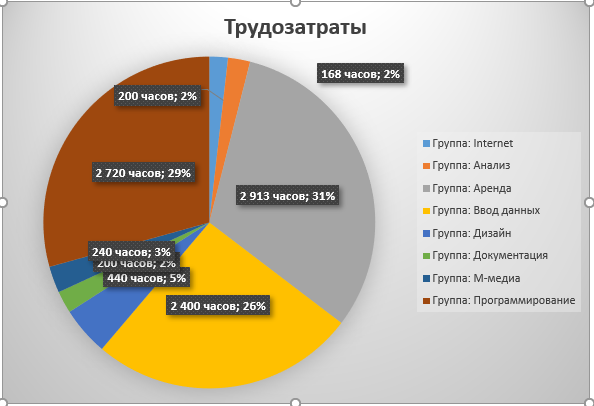
\includegraphics[width=0.7\linewidth]{src/lab3_3_2}
	\caption{}
	\label{fig:lab332}
\end{figure}

\begin{figure}[H]
	\centering
	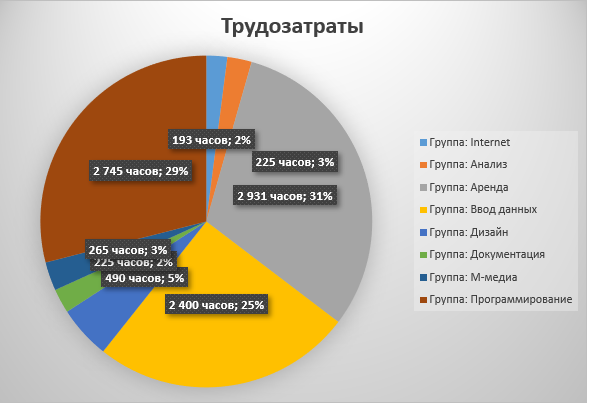
\includegraphics[width=0.7\linewidth]{src/lab3_3_3}
	\caption{}
	\label{fig:lab333}
\end{figure}

\begin{enumerate}
	\item Программирование: 2745 vs 2720
	\item Аренда: 2931 vs 2913
	\item Дизайн: 490 vs 440
\end{enumerate}

Как мы можем видеть трудозатраты выросли

\section{Заключение}
В ходе данной лабораторной работы мы научились оптимизировать ресурсы. Сокращать критический путь.
В результате данной лабороторной работы удалось продолжительность удалось сократить на 19 дней и уложиться в 47629р при бюджете в 50000


















